I often say that I am at a loss. That is somewhat common due to living
here in Ashtabula County. Daily life here is often astounding to
external observers. Picture
\href{https://en.wikipedia.org/w/index.php?title=The_Archers&oldid=1130700473}{\emph{The
Archers}} but in a warped yet dark version and you would pretty much
have Ashtabula County lately. I end up questioning the reality of some
of the seemingly bonkers scenarios that have happened lately in the
community.

It looks like we simply do not have the resource base to stand up
streaming. This happens when you're working out of your home. I don't
have office space to work out of and renting anywhere would be
cost-prohibitive.

This doesn't mean the video news plan is off, though. This means we end
up having to switch to the backup plan. We \emph{can} do video
podcasting (vodcasting) out of available resources. We can start with at
least reading the zone forecast from the National Weather Service and
showing the national surface fronts forecast chart.

\pandocbounded{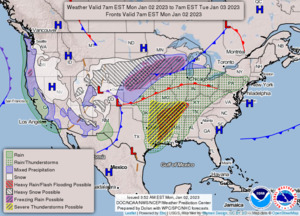
\includegraphics[keepaspectratio]{\%7B\%7Bsite.url\%7D\%7D/img/example-chart.jpg}}
\href{https://www.wpc.ncep.noaa.gov/national_forecast/natfcst.php}{\emph{available
from here}}

We're able to pull the ``Ashtabula Lakeshore'' zone forecast from
\texttt{https://tgftp.nws.noaa.gov/data/forecasts/zone/oh/ohz089.txt} to
have the material to read out. Reading that out while the surface fronts
map are displayed on-screen wouldn't be all that much but it would be
\emph{a start} compared to the lack of localized material we're getting
from our present media outlets. The ``Ashtabula Inland'' zone forecast
is found at
\texttt{https://tgftp.nws.noaa.gov/data/forecasts/zone/oh/ohz014.txt} if
we wanted to include that as well. We wouldn't immediately be using the
charts found at
\texttt{https://tgftp.nws.noaa.gov/fax/Amaster\_index.html}.

Could we add in local news coverage? Eventually we could do that. Right
now we simply do not have the staff resources to pull that off as we
would actually need people covering events. There would be interim
actions possible to pull in wire content, though. I \emph{could} tag in
newscasts
\href{https://www.dvidshub.net/search/?q=&filter\%5Btype\%5D=video&filter\%5Bcategory\%5D=Newscasts&view=grid&sort=publishdate}{taken
from the Defense Visual Information Distribution System} among the
\href{https://www.dvidshub.net/search/?q=&filter\%5Btype\%5D=video&view=grid&sort=publishdate}{other
video items they have posted} that are otherwise public domain content.
Eventually I would work in material from
\href{https://mediahelpingmedia.org/strategy/content-sharing-for-the-benefit-of-all/}{Open
Newswire} and \href{https://www.publicnewsservice.org/}{Public News
Service}. Heck, I could get statewide news from the
\href{https://www.publicnewsservice.org/state-ohio/OH}{Ohio News
Connection} that is run by
\href{https://www.publicnewsservice.org/}{Public News Service}.

This would be an effort that builds incrementally. On Monday our local
daily newspaper posted a single local news story. The paper has only
been averaging 8-12 broadsheet pages. Even though I can access the Great
Lakes Portal for information that doesn't mean most people locally can
do that effectively. Meeting information needs so that people don't rely
on rumor and innuendo spreading on Facebook is a challenge for 2023 that
might actually produce some social goods.

Right now it is more important to be putting some content out there than
to be focusing on fundraising. Fundraising would come down the road
anyhow. It certainly would be easier with a viewership of some sort.
